\documentclass{standalone}
\usepackage{tikz}
\usepackage{amsmath}

\begin{document}
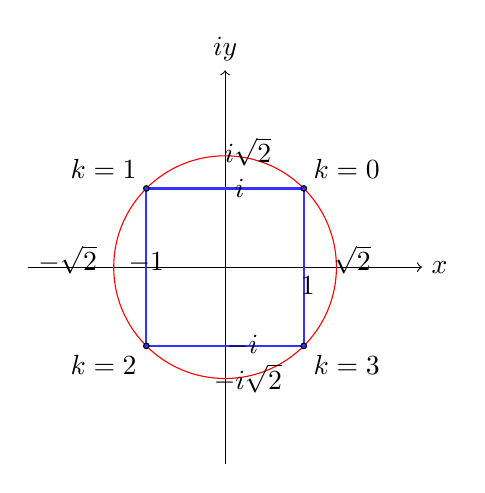
\begin{tikzpicture}[scale=1]

  % Axes
  \draw[->] (-2.5,0) -- (2.5,0) node[right] {$x$};
  \draw[->] (0,-2.5) -- (0,2.5) node[above] {$iy$};

  % Define the radius of the circle
  \def\r{sqrt(2)}

  % Circle
  \draw[red] (0,0) circle (\r);

  % Square (coordinates calculated based on the radius)
  \draw[blue!80, thick] (1,1) -- (-1,1) -- (-1,-1) -- (1,-1) -- cycle;

  % Points and labels for the square's vertices
  \draw[fill=blue!80] (1,-1) circle (1pt) node[below right] {$k=3$};
  \draw[fill=blue!80] (1,1) circle (1pt) node[above right] {$k=0$};
  \draw[fill=blue!80] (-1,--1) circle (1pt) node[above left] {$k=1$};
  \draw[fill=blue!80] (-1,-1) circle (1pt) node[below left] {$k=2$};


%   \foreach \i in {-1,1,\r, -\r-1} \draw (\i,0)--(\i,.1);

  % Labels on the axes
  \node[below ] at (1.05,0) {$1$};
  \node[above ] at (-1,-0.2) {$-1$};
  \node[right ] at (0,1) {$i$};
  \node[right] at (-0.1,-1) {$-i$};

    % Labels on the circle
    \node[] at ({\r+0.2},{0.09}) {$\sqrt{2}$};
    \node[left] at ({-\r-0.09},{0.09}) {$-\sqrt{2}$};
    \node[] at ({0.29},{\r+0.05}) {$i\sqrt{2}$};
    \node[ ] at ({0.29},{-\r}) {$-i\sqrt{2}$};

\end{tikzpicture}
\end{document}